Recombinant protein production is widely used in scientific research and industry. However, in general, the success rate of these experiments is around a 25\%, the 75\% failure rate is attributed to protein expression and solubility. In this work, we studied the major factors affecting these two steps and used the findings to develop methods to optimise the protein production. In addition, since many recombinant proteins of interest are secretory, translocation efficiency also plays an important role in the final yield. Since protein translocation is usually performed by signal peptides, fusing appropriate signal peptide to the protein of interest increases the yield. Therefore, we also developed tool to predict the presence of signal peptide in the sequence and identify the mature peptide. 

\section{Optimising protein expression using TIsigner (Translation Initiation coding region designer)}
We have demonstrated that mRNA accessibility is a better predictor of protein expression across several datasets (Table \ref{tab:Summary_of_TIsigner_and_SoDoPE}). Therefore, we used this feature to develop, TIsigner (\href{https://tisigner.com/tisigner}{https://tisigner.com/tisigner}), a tool for optimising protein expression. TIsigner uses a simulated annealing algorithm to provide a novel mechanism for tuning the protein expression from low to high levels. Other unique features include an estimation of protein expression for mRNA sequences, which we've named as 'expression score' and synonymous changes limited to the first 10 codons of the input sequence. TIsigner's synonymous substitution algorithm is designed to make a minimal number of changes. This approach is advantageous for two reasons\textemdash first, it is possible to do a PCR cloning using the optimised part as primers, which in turn reduces the cost of the experiment significantly as compared to the conventional full gene synthesis method. Second, it reduces the possibility of generating toxic mRNA sequences. mRNA toxicity is still a difficult problem to address and the mechanisms of toxicity are not fully understood yet \cite{mittal2018codon}. However, TIsigner offers a possibility to do synonymous changes over all codons, which may be useful if terminators are found. The web-version of TIsigner automatically suggests doing a full length substitution if any terminators are found (Figure \ref{fig:terminator_prompt}).

\begin{figure}[htbp!]
\center
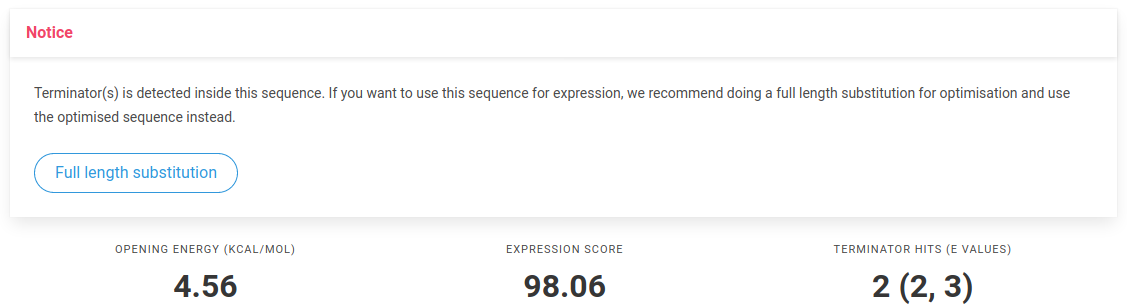
\includegraphics[width=1\textwidth]{chapters/Discussion/Figures/terminator_prompt.png}
\caption[TIsigner suggests to do a full length substitution if any transcription terminators are found in the sequence.]{\textbf{TIsigner suggests to do a full length substitution if any transcription terminators are found in the sequence.} Mock data was used for demonstration purposes.}%the List of Figures because of the *}
\label{fig:terminator_prompt}
\end{figure}


\section{Optimising protein solubility using SoDoPE (Soluble Domains for Protein Expression)}
Almost all use cases of protein require a soluble product. Hence, optimising just protein expression is not sufficient for a better protein production. Based on protein structural flexibility, which is the most accurate predictor of solubility among all conventional features, we have developed a new metric called the Solubility-Weighted Index (SWI). SWI is a very accurate predictor of solubility and outperforms other tools (Table: \ref{tab:Summary_of_TIsigner_and_SoDoPE}). Using SWI, we developed a solubility prediction and optimisation tool, SoDoPE (\href{https://tisigner.com/sodope}{https://tisigner.com/sodope}). SoDoPE is an unparalleled tool with a distinctive interface for an easy navigation of protein sequence/domains with real-time solubility prediction and optimisation. The effect of different solubility tags on solubility can also be compared to pick the best one for experiment.


\section{Detection of signal peptides using Razor}
The presence of signal peptides should almost always be checked when planning expression experiments for uncharacterised proteins. Based on the properties of signal sequences, we developed Razor (\href{https://tisigner.com/razor}{https://tisigner.com/razor}) to detect the presence of N-terminal signal peptides. Compared to other related tools, Razor also predicts toxin and fungi\textemdash specific SPs. These would be helpful for users in choosing the expression and purification systems that prevent the harmful intracellular accumulation of recombinant secretory proteins/toxins. The performance summary of Razor is given in Table \ref{tab:Summary_of_Razor}.



\section{Reception of tools by the community}
TISIGNER (\href{https://tisigner.otago.ac.nz}{https://tisigner.otago.ac.nz}, \href{https://tisigner.com}{https://tisigner.com}, \href{https://tisigner.nz}{https://tisigner.nz}) is the web-suite for these tools. Initially, it consisted of TIsigner only, hence the name, but has been expanded to include both SoDoPE and Razor. Our tool has been online since February 2020. Despite the short period (March 2021 at the time of writing), our tools are gaining traction among researchers worldwide, with an exponential increase in the numbers of visitors from many countries (Figure \ref{fig:tisigner_stats}).


\begin{figure}[H]
\center
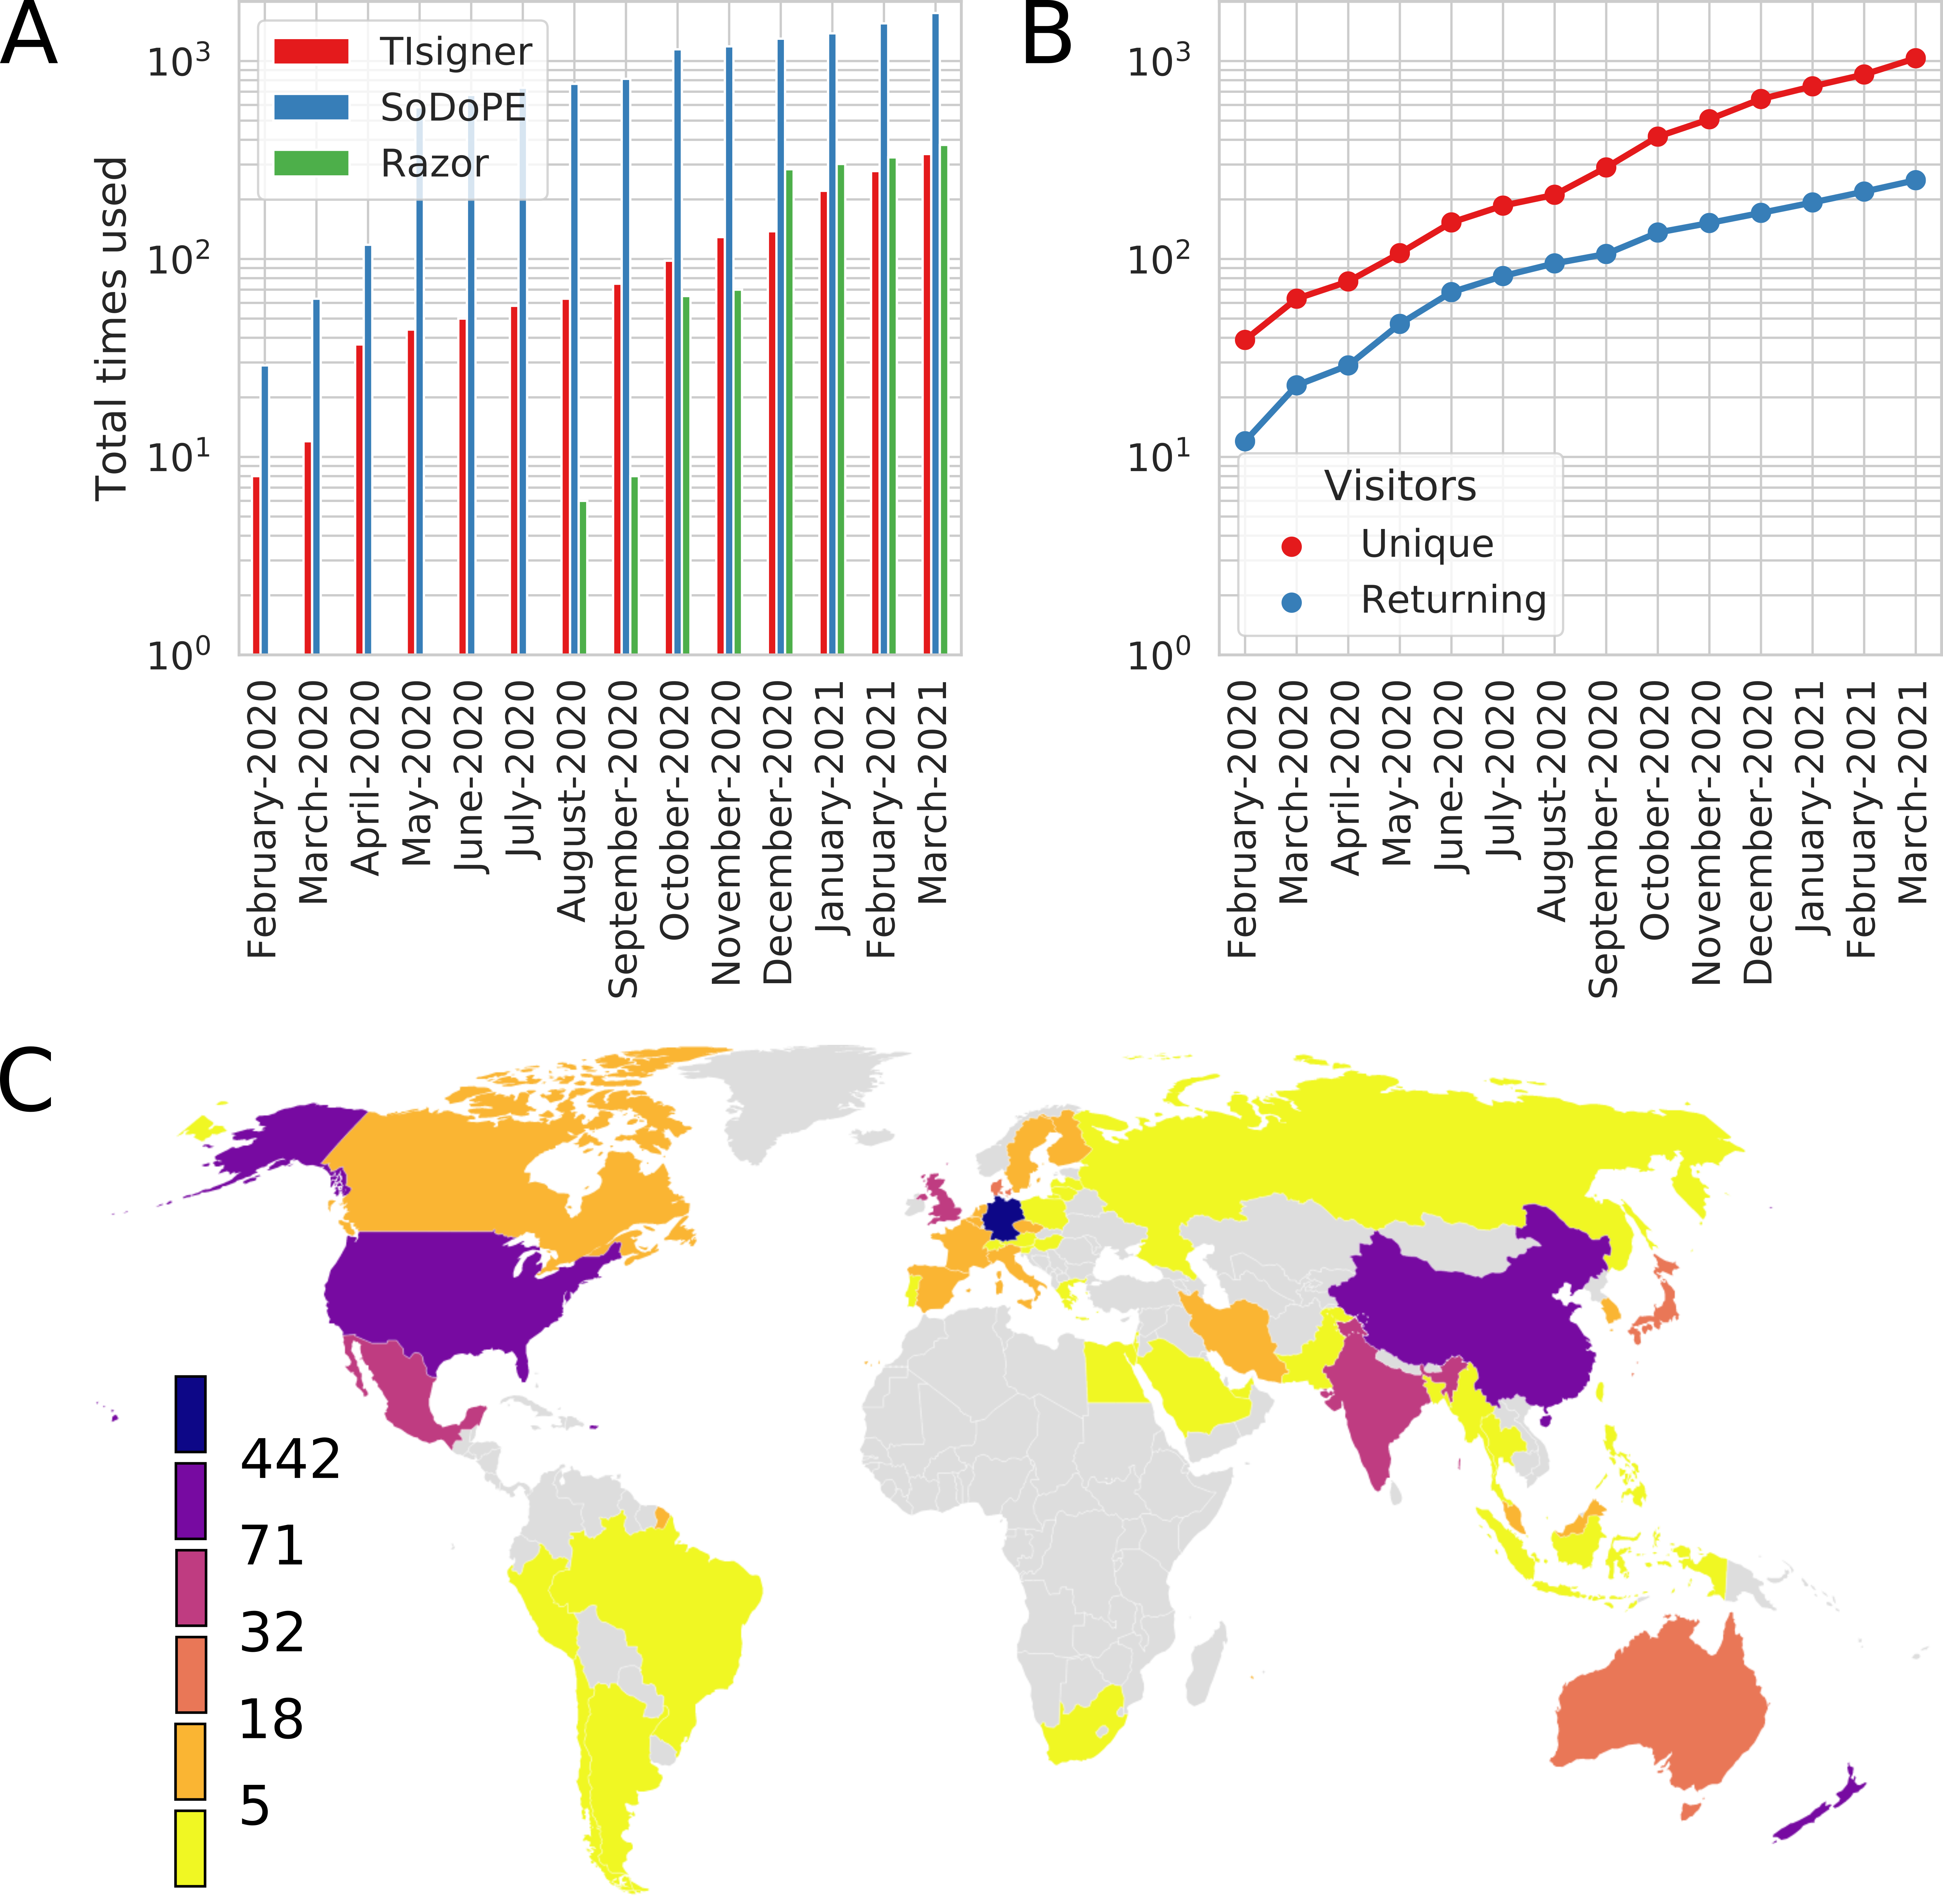
\includegraphics[width=0.8\textwidth]{chapters/Discussion/Figures/tisigner_stats.png}
\caption[TISIGNER.com web service is getting popular among researchers worldwide.]{\textbf{TISIGNER.com web service is getting popular among researchers worldwide. (A)} Number of times each tool was used in a logarithmic scale. \textbf{(B)} The number of unique and returning visitors in a logarithmic scale. \textbf{(C)} Geographical location of users. Data is for the period of February 2020 to March 2021 from Google Analytics (\href{https://analytics.google.com}{https://analytics.google.com}). }%the List of Figures because of the *}
\label{fig:tisigner_stats}
\end{figure}


\section{Outlook}
Tthe present work enumerates some of the cellular level processes responsible in protein synthesis. In this section, we will use a simplified version of higher level modelling by taking into account of the production system as a black-box (S) which has various levels of noise and uncertainties. In such a crowded environment, there might be some, possibly unknown, additional constrain and feedback between or within the cells, which could stabilise or destabilise the production system. Let us represent any and all of these uncertainties, noises and feedbacks collectively by a black-box (F) and simply refer to as feedbacks. A stable system is a result of interplay between the system and its feedback. These type of systems are called \textit{control systems} (Figure \ref{fig:control_system}A). The output behaviour of output of these systems when the input is switched from low to high is studied within the framework of step response.

\begin{figure}[htbp!]
\center
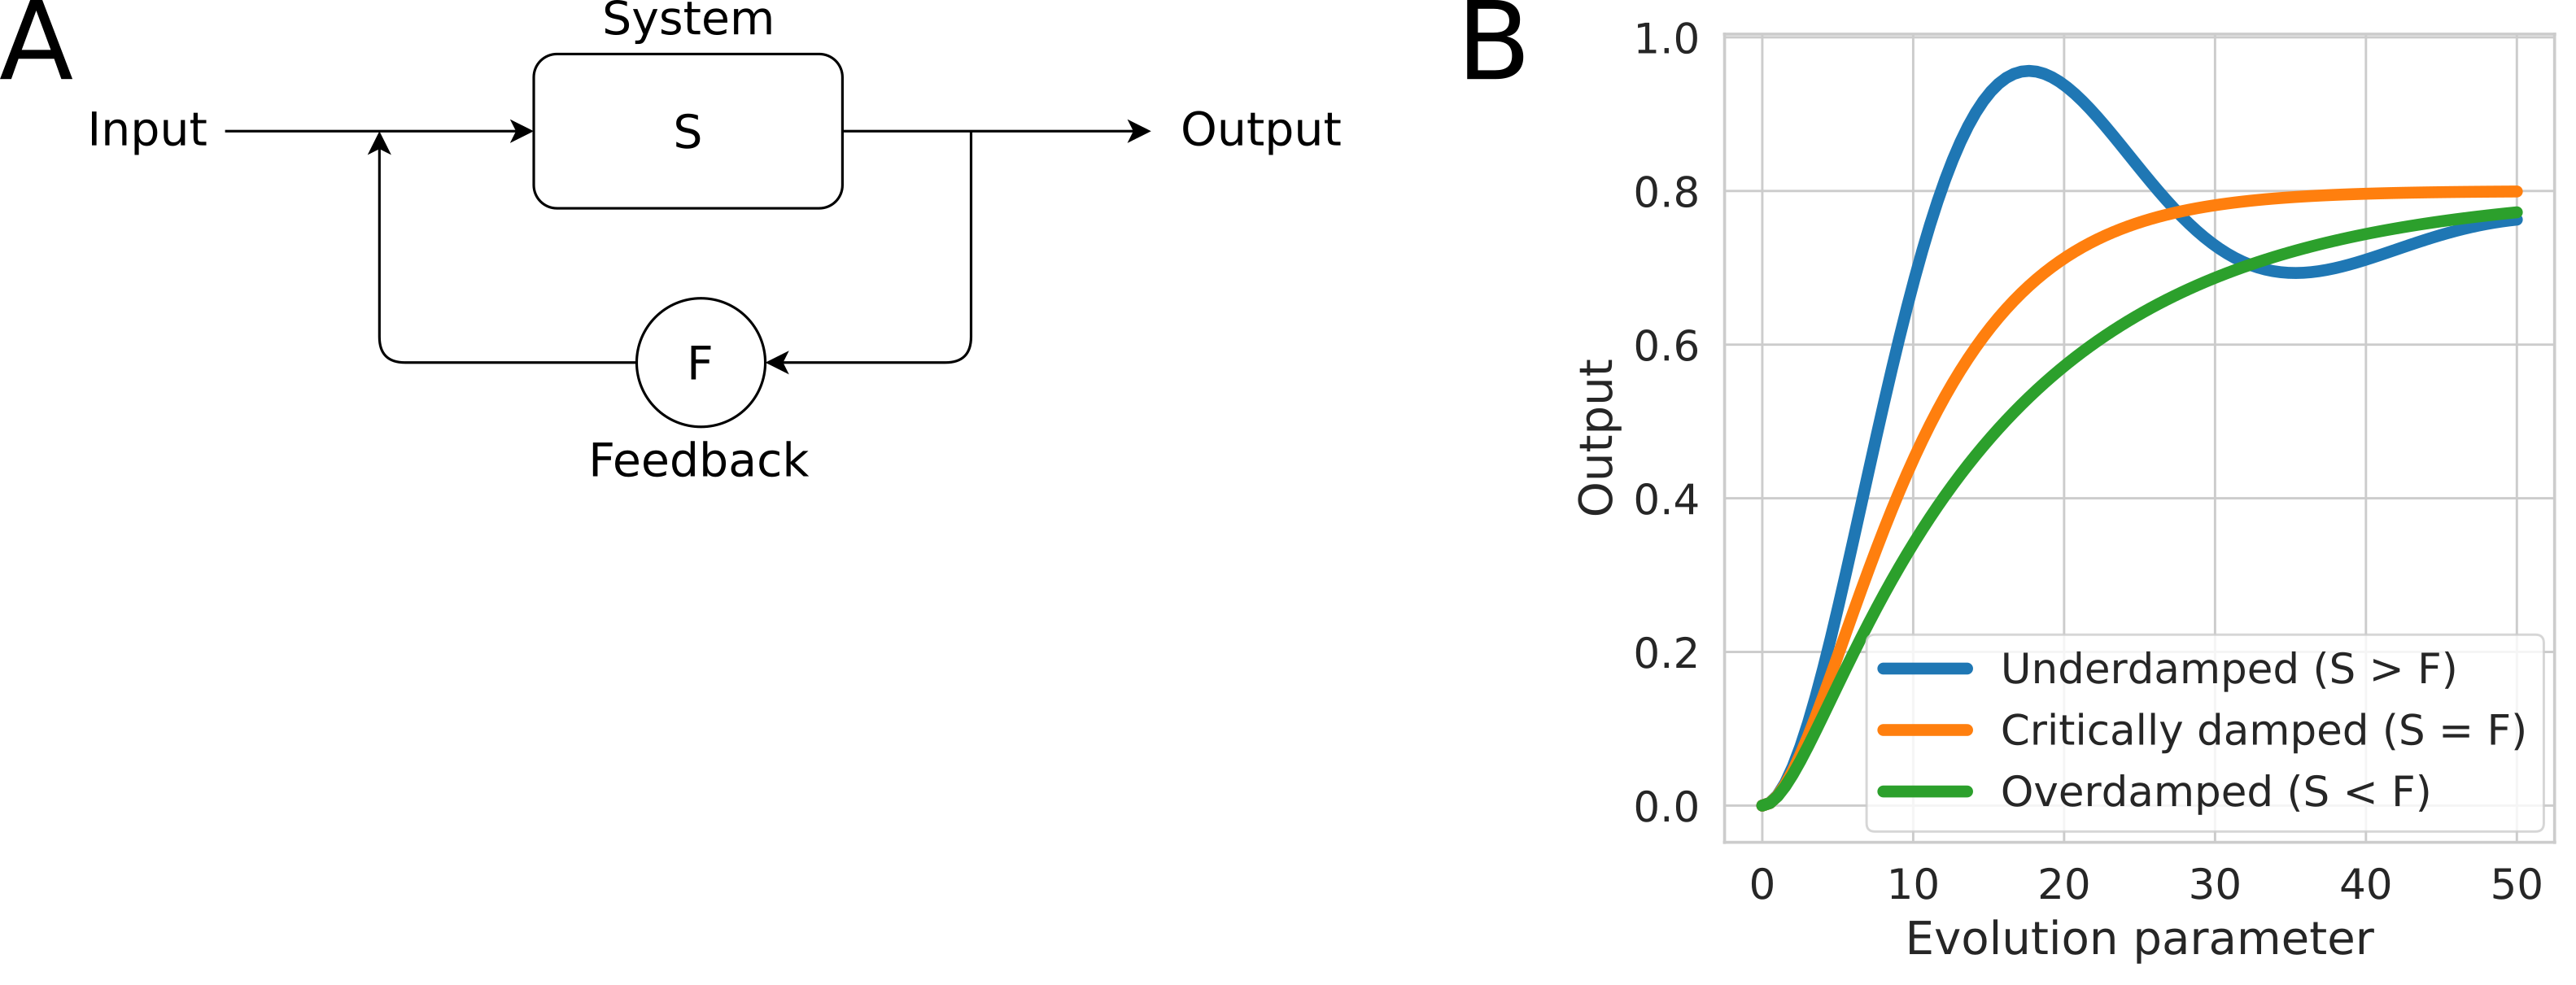
\includegraphics[width=1\textwidth]{chapters/Discussion/Figures/control_system.png}
\caption[Different possible step responses of a stable control system when input is switched from low to high.]{\textbf{Different possible step responses of a stable control system when input is switched from low to high. (A)} A control system (S) with a feedback loop (F). This system is assumed to be stable. \textbf{(B)} Output (step response) when the damping effects due to feedback (F) are low, equal and high compared to the system (S). Evolution parameter is an arbitrary parameter of the system.}%the List of Figures because of the *}
\label{fig:control_system}
\end{figure}

In control theory, the evolution of higher order system with respect to some evolution parameter (often time, but could be any other variable) is approximated by a second order ordinary differential equation: 
\begin{equation}
    \Ddot{x} + 2\zeta\omega_n\dot{x} + \omega_n^2 x = 0
\end{equation}
where $\omega_n$ is the eigen frequency, $\zeta$ is the damping ratio. The eigen frequency is the frequency at which the system oscillates when no external forces are present, whereas damping ratio is an indicative of the relative strength of feedback to the system (F/S). The most general solution of this equation can be written as a linear combination:
\begin{equation}
    x = Ce^{-\omega_n(\zeta + i\sqrt{1-\zeta^2})} + De^{-\omega_n(\zeta - i\sqrt{1-\zeta^2})}
\end{equation}

Hence for any system, multiple output possibilities exist which are shown in Figure \ref{fig:control_system}B. For $0 \leq \zeta < 1 $, the output is decaying exponential with oscillations and is called underdamped. For $\zeta > 1$, the system does not oscillate and is called overdamped whereas for $\zeta = 1$, the system is logistic in nature and is called critically damped. 



% Documents/Thesis/Committee_Meeting_April_2020/Jupyter_Notebook/NonLinearRegression/For_Thesis.ipynb
\begin{wrapfigure}{r}{0.5\textwidth}
  \begin{center}
    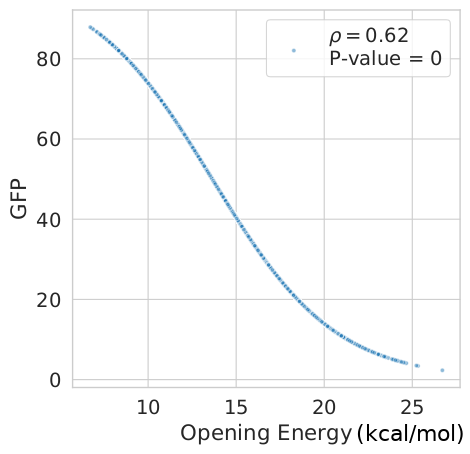
\includegraphics[width=0.5\textwidth]{chapters/Discussion/Figures/cambray_fitting.png}
    \caption[Best fit shows an overdamped ($\zeta > 1$) trend in GFP data from Cambray \textit{et al.}]{\textbf{Best fit shows an overdamped ($\zeta > 1$) trend in GFP data from Cambray \textit{et al.} (2018)} Spearman's $\rho = 0.62$, P-value is less than machine's underflow. In these type of systems, the output increases steadily with an increase in input level. Reverse trend is because lower opening energy are more optimal than higher opening energy sequences. }%the List of Figures because of the *}The opening energy of the region (-24:24) is used.
    \label{fig:refitting_data_cambray}
  \end{center}
\end{wrapfigure}

Ideally, physical systems with $\zeta = 1$ (critically damped) are preferred because the maximum output can be reached easily. In contrast, biological systems are often noisy, which could make the output behave like either of the cases. As an illustration, the data from Cambray \textit{et al.} \cite{Cambray2018-kn}, follows an overdamped trend ($\zeta > 1$) (Figure \ref{fig:refitting_data_cambray}). However, the results of our GFP experiments using TIsigner, fits better to the underdamped system ($0 \leq \zeta < 1 $) than a logistic regression (critically damped) (Figure \ref{fig:refitting_data_tisigner}). In this case, the output tends to oscillate when the input is increased beyond a certain limit, which we observed (Figure \ref{fig:refitting_data_tisigner}C).


% Documents/Thesis/Committee_Meeting_April_2020/Jupyter_Notebook/NonLinearRegression/For_Thesis.ipynb
\begin{figure}[htbp!]
\center
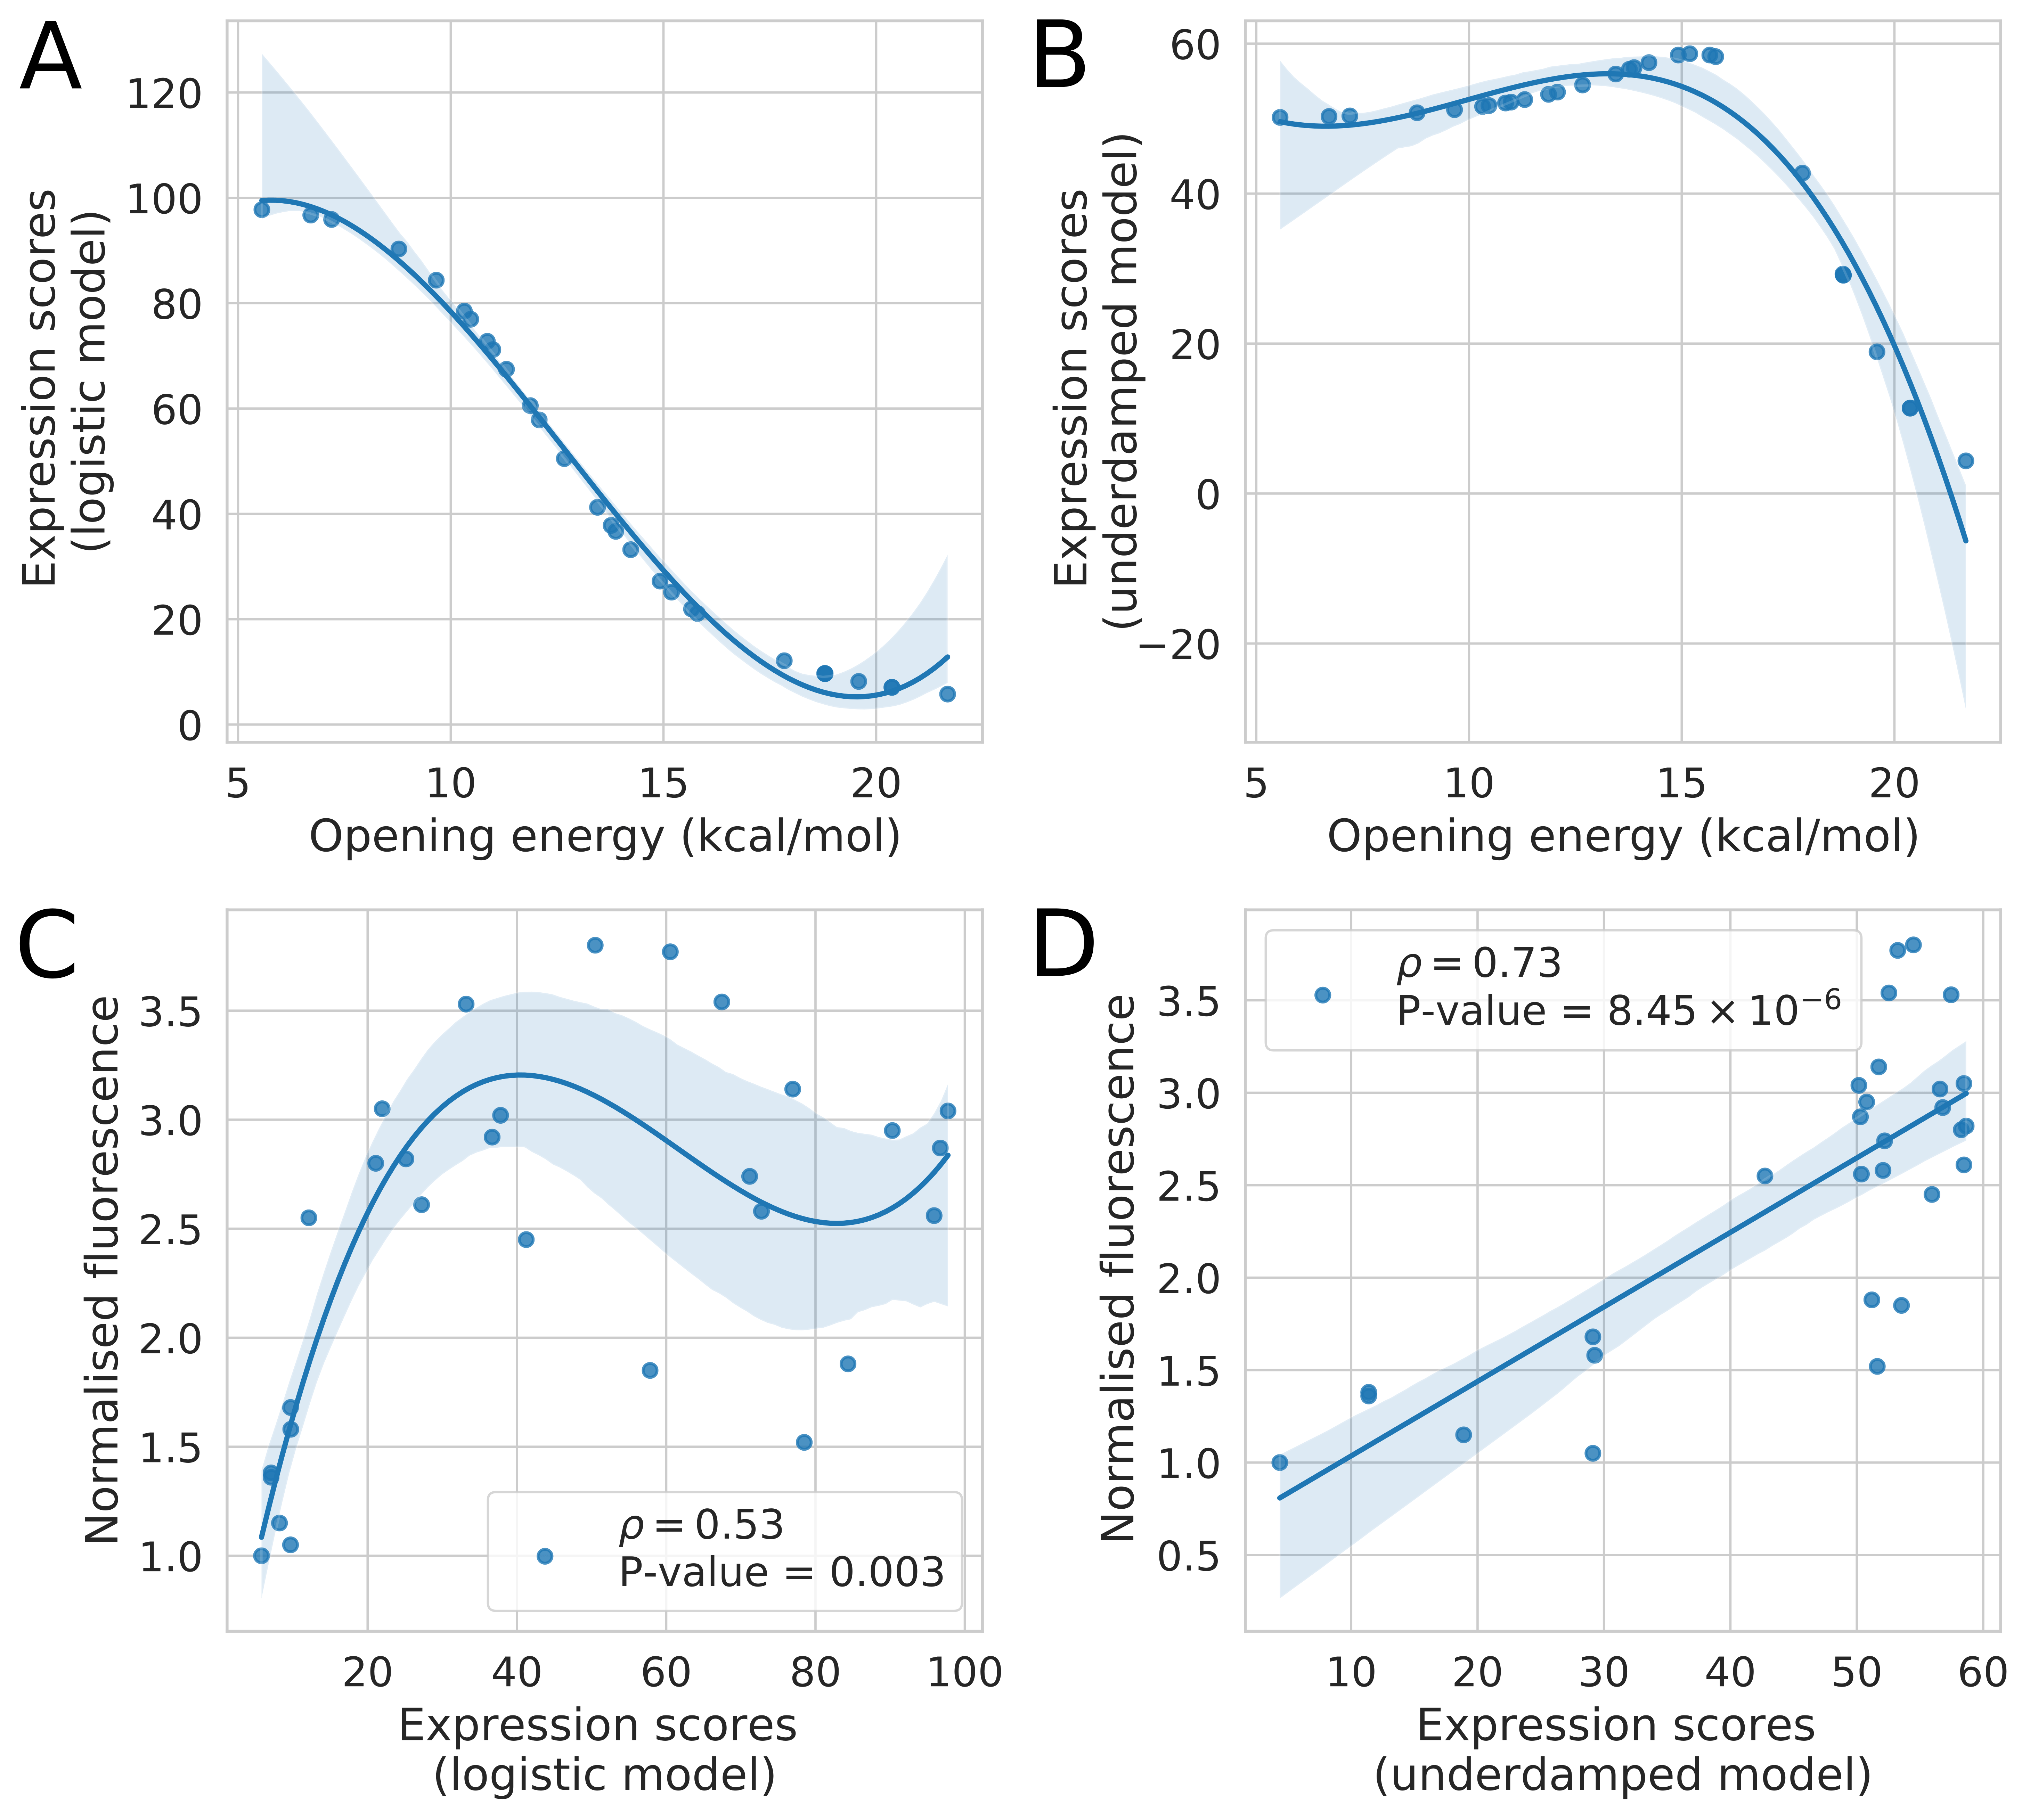
\includegraphics[width=0.9\textwidth]{chapters/Discussion/Figures/refitting_tisigner.png}
\caption[An underdamped model fits better to the TIsigner experimental data (GFP) than a logistic (critically damped) model.]{\textbf{An underdamped model fits better to the TIsigner experimental data (GFP) than a logistic (critically damped) model.} The conversion of opening energy to expression score using \textbf{(A)} logistic (critically damped) model and  \textbf{(B)} underdamped model. Spearman'r $\rho$ between normalised fluorescence and expression scores derived from \textbf{(C)} logistic model and \textbf{(D)} underdamped model. Spearman's $\rho$ is stronger when we model the production as underdamped (0.73, P-value=$8.45\times 10^{-6}$) compared to the critically damped model (0.53, P-value=0.003). Lines represent the best fit regression.}%the List of Figures because of the *}
\label{fig:refitting_data_tisigner}
\end{figure}

 These inherent and inevitable feedbacks and constrains, for example protein toxicity and solubility issues, may be different for different systems, protein of interest and protocols. In this work, these issues were treated separately. However, modelling the production system by taking into account of all these variables may be required to explain the outcomes of recombinant protein production systems with a greater accuracy. The simulated production system (Fig \ref{fig:tisigner_fig4}), which takes into account of only the protein toxicity and mRNA accessibility, was surprisingly close to the experimental results. Combined with a higher order modelling as outlined above, such simulations can be used to explore and study the effects of different features of mRNA and protein as well as stochasticity. Nevertheless, this work provides a sufficient background for such a complex modelling in the future.
 
 
%  The results from the simulation in (Fig \ref{fig:tisigner_fig4}), which takes into account of protein toxicity and mRNA accessibility, was surprisingly close to the experimental results. Such simulations and modelling can be used to explore the effects of many mRNA and protein features as well as stochasticity. Nevertheless, this work provides a sufficient background for such complex modelling in the future. 
 
   


% \section{Future work and outlook}
